%; whizzy paragraph -pdf xpdf -latex ./whizzypdfptex.sh
%; whizzy-paragraph "^\\\\begin{frame}"
% latex beamer presentation.
% platex, latex-beamer でコンパイルすることを想定。 

%     Tokyo Debian Meeting resources
%     Copyright (C) 2011 Junichi Uekawa
%     Copyright (C) 2011 Nobuhiro Iwamatsu

%     This program is free software; you can redistribute it and/or modify
%     it under the terms of the GNU General Public License as published by
%     the Free Software Foundation; either version 2 of the License, or
%     (at your option) any later version.

%     This program is distributed in the hope that it will be useful,
%     but WITHOUT ANY WARRANTY; without even the implied warreanty of
%     MERCHANTABILITY or FITNESS FOR A PARTICULAR PURPOSE.  See the
%     GNU General Public License for more details.

%     You should have received a copy of the GNU General Public License
%     along with this program; if not, write to the Free Software
%     Foundation, Inc., 51 Franklin St, Fifth Floor, Boston, MA  02110-1301 USA

\documentclass[cjk,dvipdfmx,12pt]{beamer}
\usetheme{Tokyo}
\usepackage{monthlypresentation}

%  preview (shell-command (concat "evince " (replace-regexp-in-string  "tex$" "pdf"(buffer-file-name)) "&")) 
%  presentation (shell-command (concat "xpdf -fullscreen " (replace-regexp-in-string "tex$" "pdf"(buffer-file-name)) "&"))
%  presentation (shell-command (concat "evince " (replace-regexp-in-string "tex$" "pdf"(buffer-file-name)) "&"))

%http://www.naney.org/diki/dk/hyperref.html
%日本語EUC系環境の時
\AtBeginDvi{\special{pdf:tounicode EUC-UCS2}}
%シフトJIS系環境の時
%\AtBeginDvi{\special{pdf:tounicode 90ms-RKSJ-UCS2}}

\title{月刊 debhelper 第1回}
\subtitle{第81回 2011年10月度}
\author{岩松 信洋 iwamatsu@debian.org\\IRC nick: iwamatsu}
\date{2011年10月22日}
\logo{
\includegraphics[width=8cm]{image200607/openlogo-light.eps}}

\begin{document}

\frame{\titlepage{}}


\begin{frame}{自己紹介}
省略。
\end{frame}


\begin{frame}{アジェンダ}
\begin{enumerate}
\item debhelper とは?
\item 月刊 debhelperとは?
\item debian パッケージ構築、全体の流れ
\item 今月のコマンド : その1
\item 今月のコマンド : その2
\item 大事なお知らせ
\end{enumerate}
\end{frame}

\begin{frame}{debhelperとは?}

\begin{itemize}
\item Debian パッケージを作る際に必要な機能をまとめたツール。
\item 他にも同様のツールがいくつかありますが、1番使われているのがこの debhelper。
\item Debian パッケージをメンテナンスしている人にとって debhelper の知識が必須と
言ってもいい。
\item 開発者は Debian 開発者の Joey Hess 氏
\item 最新のバージョンは 8.9.8
\end{itemize}
\end{frame}



\begin{frame}{月刊debhelperとは?}

\begin{itemize}
\item Debian パッケージをメンテナンスしている人にとって debhelper の知識が必須。
\item しかし提供されるコマンドが多い。しかも、最近は省略していてなにやっているのか
わからん。
\end{itemize}
\end{frame}


\begin{frame}[containsverbatim]{debian パッケージ構築、全体の流れ}
\begin{multicols}{2}

\begin{commandline}
debhelper 6:
#!/usr/bin/make -f

build: build-stamp
build-stamp:
    dh_testdir
    $(MAKE)
    touch $@

clean:
    dh_testdir
    dh_testroot
    $(MAKE) clean
    dh_clean

install: build
    dh_testdir
    dh_testroot
    dh_clean -k

binary-indep:

binary-arch: build install
    dh_testdir
    dh_testroot
    dh_installchangelogs ChangeLog
    dh_installd
.....
\end{commandline}
\columnbreak
\begin{commandline}
debhelper 7:
#!/usr/bin/make -f
%:
        dh $@
\end{commandline}
\end{multicols}
% $
\end{frame}


\begin{frame}{月刊debhelperとは?}
\begin{itemize}
\item 毎月数個づつ紹介してちょっとづつ理解していこう。
\item 全部終わっているころには、Debian パッケージメンテナ担っているかもしれない!?
\end{itemize}
\end{frame}

\emtext{debian パッケージ構築、全体の流れ}

\begin{frame}{debian パッケージ構築、全体の流れ}
\begin{enumerate}
\item パッケージビルド環境を構築する
\item 不要なファイルを削除する
\item バイナリパッケージに格納するファイルをビルドする
\item ビルドしたファイルをバイナリパッケージにまとめる
\item .changesファイルを作成する
\item パッケージに署名する
\end{enumerate}
\end{frame}

\begin{frame}{1. パッケージビルド環境を構築する}
\begin{itemize}

\item ソースコードの展開
\item パッケージ構築依存のチェック

\end{itemize}
\end{frame}

\begin{frame}[containsverbatim]{2. 不要なファイルを削除する}
\begin{itemize}

\item 前に行われたパッケージビルドで生成されたファイルの削除します。
\item ソースが展開された常に同じ状態からビルドできるようにします。
\item debian/rules の clean ターゲットで行われる必要があり、これは
Debian Policy で決まっています。
\item 以下のdebhelper コマンドが実行されます。
\begin{commandline}
dh_testdir -> dh_auto_clean -> dh_clean
\end{commandline}

\end{itemize}
\end{frame}

\begin{frame}[containsverbatim]{3. バイナリパッケージに格納するファイルをビルドする}
\begin{itemize}

\item ビルド前の設定を行います。configureの実行など。
\item 実際のビルドを行います。
\item pdf等のドキュメントの生成もここで行われます。
\item debian/rules の build ターゲットで行われる必要があり、これは
Debian Policy で決まっています。
\item 以下のdebhelper コマンドが実行されます。
\begin{commandline}
dh_testdir -> dh_auto_configure -> dh_auto_build -> dh_auto_test
\end{commandline}

\end{itemize}
\end{frame}

\begin{frame}[containsverbatim]{4. ビルドしたファイルをバイナリパッケージにまとめる}
\begin{itemize}

\item 必要なファイルをすべてビルド完了した後、それらを適切なパーミッションで
適切な場所に配置し、バイナリパッケージにまとめます。

\item debian/rules の binary、binary-arch、 binary-indep ターゲット
で行われる必要があり、これは
Debian Policy で決まっています。
\end{itemize}
\end{frame}

\begin{frame}[containsverbatim]{4. ビルドしたファイルをバイナリパッケージにまとめる}
\begin{itemize}

\item 以下のdebhelper コマンドが実行されます。
\begin{commandline}
dh_testdir -> dh_auto_configure -> dh_auto_build -> dh_auto_test
-> dh_testroot -> dh_prep -> dh_installdirs -> dh_auto_install
-> dh_install -> dh_installdocs -> dh_installchangelogs
-> dh_installexamples -> dh_installman -> dh_installcatalogs
-> dh_installcron -> dh_installdebconf -> dh_installemacsen
-> dh_installifupdown -> dh_installinfo -> dh_pysupport
-> dh_installinit -> dh_installmenu -> dh_installmime
-> dh_installmodules -> dh_installlogcheck -> dh_installlogrotate
-> dh_installpam -> dh_installppp -> dh_installudev -> dh_installwm
-> dh_installxfonts -> dh_installgsettings -> dh_bugfiles -> dh_ucf
-> dh_lintian -> dh_gconf -> dh_icons -> dh_perl -> dh_usrlocal
-> dh_link -> dh_compress -> dh_fixperms -> dh_strip -> dh_makeshlibs
-> dh_shlibdeps -> dh_installdeb -> dh_gencontrol -> dh_md5sums
-> dh_builddeb
\end{commandline}

\end{itemize}
\end{frame}

\begin{frame}[containsverbatim]{5. .changesファイルを作成する}
\begin{itemize}

\item  パッケージの.changelog ファイルを作成します。
\item ファイルの作成には dpkg-genchanges コマンドが使われます。
\item コマンドは debhelper のコマンドではありません。

\end{itemize}
\end{frame}

\begin{frame}[containsverbatim]{6. パッケージに署名する}
\begin{itemize}

\item .dscファイルと.changes ファイルにGPG/PGPを使って署名をします。
\item この署名には debsign コマンドを使います。
\item このコマンドは debhelper のコマンドではありません。
\end{itemize}
\end{frame}

\begin{frame}{debian パッケージ構築、全体の流れ}

\begin{figure}[ht]
  \begin{center}
    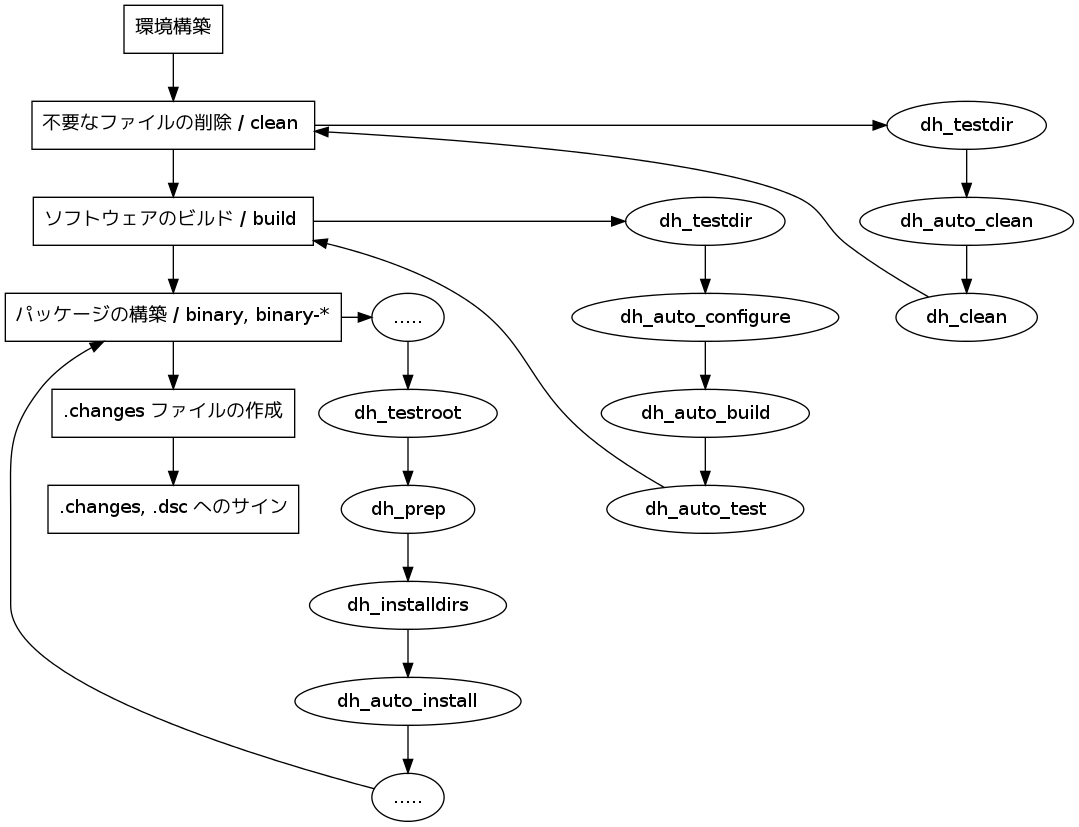
\includegraphics[height=8cm]{image201110/rules-work.png}
  \end{center}
\end{figure}
\end{frame}

\emtext{その他 debhelper の重要な機能}

\begin{frame}[containsverbatim]{環境にあわせたシーケンス情報を読み込む}
debhelper は特定の言語や環境に合わせたシーケンスを定義し、
読み込ませることによって、makefile 内で利用できるターゲットと
コマンドを増やすことができます。

使いたい場合には、{\bf --with}オプションを使って指定します。

quiltの例:
\begin{commandline}
%:
        dh $@ --with quilt
\end{commandline}
%$
指定することによって、\bf{dh\_quilt\_patch}が利用できるようになります。
\end{frame}

\begin{frame}[containsverbatim]{各 debhelper コマンドの動きを変更する}
上記で説明しように、debhelper では各ターゲットと
各コマンドの動作が予め決められています。
これらを変更するには各コマンド用のターゲットに対して動作を記述します。
このターゲットは {\bf override\_各debhelper コマンド}となっており、dh\_auto\_configure
(決められた値で自動的に configure を実行するためのコマンド)の場合には以下のように使います。

\begin{commandline}
......
override_dh_auto_configure:
    dh_auto_configure -- --enable-foo
......
\end{commandline}


\end{frame}


\emtext{今月のコマンド}

\begin{frame}{今月のコマンド : dh\_testdir}
\begin{itemize}
\item 概要\\
パッケージビルドを行うときに正しいディレクトリにいるかチェックします。
\end{itemize}
\end{frame}

\begin{frame}[containsverbatim]{今月のコマンド : dh\_testdir}
\begin{itemize}
\item 使い方\\

dh\_testdir コマンドはカレントディレクトリに debian/control があることに
よって正しいディレクトリにいるかチェックをしています。
dh\_testdir はほとんどのターゲットから利用されます。ちゃんと debian パッケージ
をビルドできる場所にいるかチェックするためです。

\end{itemize}

\begin{commandline}
$ mkdir foo
$ cd foo
$ dh_testdir
dh_testdir: cannot read debian/control: そのようなファイルやディレクトリはありません
echo $?
2
$ mkdir debian
$ touch debian/control
$ dh_testdir
$ echo $?
0
\end{commandline}
%$
\end{frame}

\begin{frame}[containsverbatim]{今月のコマンド : dh\_testdir}
\begin{itemize}
\item 使い方\\
引数としてファイルパスを指定することができます。
ファイルパスを指定した場合には、指定したファイルによってチェックが行われます。
\end{itemize}

\begin{commandline}
$ touch moo
$ dh_testdir moo
$ echo $?
0
\end{commandline}
%$
\end{frame}

%----------------------------------------------------------------------------

\emtext{今月のコマンド}

\begin{frame}{今月のコマンド : dh\_bugfiles}
\begin{itemize}
\item 概要\\
dh\_bugfiles コマンドは バグレポートに必要なファイルをパッケージに
格納します。
バグレポートに使うファイルは script、control、presubj の3つがあり、
debian/bug ディレクトリに格納されている必要があります。
\end{itemize}
\end{frame}

\begin{frame}[containsverbatim]{今月のコマンド : dh\_bugfiles}
\begin{itemize}
  \item 各ファイル\\
  \begin{itemize}
    \item script

バグレポート用のスクリプトです。
バグレポートを行うためのツールreportbugs 等でレポート作成時に呼び出し、
結果をバグレポートの一部として追記します。
例えば、X.Orgのドライバ群は /usr/share/bug/xserver-xorg-core/script 
にシンボリックリングを張ったファイルをバイナリパッケージ内に持ちます。
このスクリプトでは、reportbug を実行した環境のカーネルバージョンや 
dmesg, xorg のログなどが自動的に出力されるようになっています。

  \end{itemize}
\end{itemize}
\end{frame}

\begin{frame}[containsverbatim]{dh\_bugfiles/設定ファイル}
  \begin{itemize}
  \item control\\

controlファイルは指定したコマンドの結果をバグレポートの一部として出力します。
コマンドには以下の4つがあります。

  \end{itemize}
\end{frame}
\begin{frame}[containsverbatim]{dh\_bugfiles/設定ファイル}
    \begin{itemize}
    \item package-status
指定したパッケージのステータス(インストール状態、バージョン)を
バグレポートに追加します。

\begin{commandline}
設定例:
/usr/share/bug/mutt/control package-status: mutt mutt-patched ....
\end{commandline}
    \end{itemize}
\end{frame}

\begin{frame}[containsverbatim]{dh\_bugfiles/設定ファイル}
  \begin{itemize}
    \item report-with
指定したパッケージ情報をバグレポートに追加します。

\begin{commandline}
設定例:
/usr/share/bug/xorg/control report-with: xserver-xorg
\end{commandline}

    \item Send-To
Debian BTS以外に自動的にが行われるメールアドレスを設定します。

\begin{commandline}
Send-To: foo@example.org
\end{commandline}

    \item Submit-As:
一つのパッケージにレポートが行われるようにコントールする
以下のように設定した場合、linux-image-3.0.0-2-amd64 にバグレポート
した場合には linux-2.6 に行われるように自動的に変更されます。

\begin{commandline}
control:Submit-As: linux-2.6
\end{commandline}
    \end{itemize}

\end{frame}


\begin{frame}[containsverbatim]{dh\_bugfiles/設定ファイル}
  \begin{itemize}
    \item presubj

レポートする前の警告文を出すために使います。
例えば、gnupg パッケージの場合にはこのファイルに
\begin{commandline}
Please consider reading /usr/share/doc/gnupg/README.BUGS.Debian before
sending a bug report. Maybe you'll find your problem there.
\end{commandline}
と書くことによって、バグレポートを送る前に /usr/share/doc/gnupg/README.BUGS.Debian 
を参照するよう、誘導しています。

reportbug を使って、バグレポートしようとしたとき、以下のような
メッセージが表示されます。
\begin{commandline}
Please consider reading /usr/share/doc/gnupg/README.BUGS.Debian before
sending a bug report. Maybe you'll find your problem there.


(You may need to press 'q' to exit your pager and continue using
reportbug at this point.)
\end{commandline}

\end{itemize}
\end{frame}


\begin{frame}[containsverbatim]{dh\_bugfiles/使い方}
このコマンドは install ターゲットで使用します。

\begin{commandline}
install:
    ....
    dh_bugfiles
    ....
\end{commandline}

\end{frame}

\emtext{大事なお知らせ}

\begin{frame}[containsverbatim]{大事なお知らせ}
\end{frame}

\begin{frame}{月刊 debhelper 楽しい\sout{悪魔の}ルール}

毎月数個づつ紹介するといっても、同じ人が毎回教えていては面白くありません(個人的に)。
Debian{\bf 勉強会}なので、毎月持ち回りで各 debhelper コマンドを紹介するという方法を取ります。
以下が私が勝手に決めた\sout{ひどい}とても楽しいルールです。

\end{frame}

\begin{frame}{月刊 debhelper 楽しい\sout{悪魔の}ルール}
\begin{itemize}
\item 一人2個以上の debhelper コマンドの説明をする。
\item 当月の発表者が次に発表させる人を決めることができる。
\item ただし、自分で立候補する場合はその限りではない。
\item 同じ人が続けて発表できない。最大2回空けること。
\item 勉強会に参加していない人を指定してはいけない。
\item 一番最初の発表者がルールを決めることができる(超重要。ようするに岩松)。
\end{itemize}

早く発表すると比較的簡単なものとか、自分が勉強したいものから発表できるかもしれません。
debhelper コマンド争奪戦の始まりです。

\end{frame}

\emtext{月刊 debhelper 次回の発表者}

\begin{frame}{月刊 debhelper 次回の発表者}

次回の発表者は野島さんです。おめでとうございます。
頑張ってください。

\end{frame}

\emtext{質問?}

\begin{frame}[containsverbatim]{質問?}
\end{frame}


\end{document}

;;; Local Variables: ***
;;; outline-regexp: "\\([ 	]*\\\\\\(documentstyle\\|documentclass\\|emtext\\|section\\|begin{frame}\\)\\*?[ 	]*[[{]\\|[]+\\)" ***
;;; End: ***
